% Copyright (c) 2014,2016 Casper Ti. Vector
% Public domain.

\chapter{PandaX-III项目介绍}
\label{chapter:intro}
%\pkuthssffaq % 中文测试文字。

正如上文所说的,无中微子双Beta衰变事件是一种极其稀有的事件,既有实验已经给去它的半衰期$T^{0\nu}_1/2>1.07\times10^{26}$年,需要达成给出中微子质量顺序这一中期目标至少需要1吨量级的衰变元素。因而相应的实验难点便是以下四点:
\begin{enumerate}
    \item 顺利制造生产出吨级的可能发生NLDBD事件的放射性元素。
    \item 探测器具有极佳的能量分辨率和位置分辨率,能够准确的捕捉到NLDBD事件。
    \item 探测器本底噪声很低,在灵敏区域的背景事件应该小于0.1个每吨每年。
    \item 合适的数据处理方法来区分NLDBD事件以及和背景事件
\end{enumerate}
在PandaX-III实验中我们通过适当的选择衰变元素以及合理设计构造探测器结构等诸多方法来解决上述四点难点,以此保障能够顺利的达成探测NLDBD事件的实验目标。

\section{元素选择}

在诸多可以发生 NLDBD 事件的放射性元素中,PandaX-III选取了$^{136}$Xe作为目标,因为其在自然界中含量较为丰富,因而相对便宜。再有$^{136}$Xe作为衰变元素的同时也可以作为探测器的敏感气体,因而使用它可以制造出相当巨大的气体探测器。该元素 NLDBD 事件释放出的总能量为$Q_{\beta\beta}=2458keV$,这个能量相对较高,能够避免低能的背景辐射,但是在$Q_{\beta\beta}$附近也有来自$^{214}$Bi和$^{208}$Tl两种元素 Gamma 衰变的本底噪声,其中$^{214}$Bi会产生2448keV的Gamma射线,只比$Q_{\beta\beta}$低了10keV。这两种元素作为$^{238}$U和$^{232}$Th衰变链中的中间元素广泛存在于自然界的各个角落中,因而对PandaX-III实验提出了巨大的挑战。

PandaX-III使用了10bar的高压气氙作为探测气体,其中$^{136}$Xe的丰度为90\%。同时为了配合电子学读出系统,气体混合了1\%的TMA(trimethylamine)来增强信号质量,根据NEXT实验的相关研究,使用该混合气体作为探测介质能够达到3\%的能量分辨率\supercite{azevedoh2015accurate}。

\section{探测器构造}

为了能够达到优秀的能量分辨率,Pandax-III计划建造5个200kg级别的高压气氙时间漂移室(time projection chamber, TPC)作为 NLDBD 的探测器,如图\ref{fig:detector}左所示。高压气体时间漂移室的技术在上个世纪90年代便已经成熟,相对与液体漂移时而言它能够提供更为优良的能量分辨率,如果使用直接读出电离电子数目的读取器件,高压气体TPC的分辨率能够接近达到液体的10倍。高压气体时间漂移室另外一个十分巨大的优势是能够较好的保留 NLDBD 事件的径迹,配合像素或者条状读出事件的径迹可以十分便捷的重建出,利用径迹信息可以极高效率的分辨出本地事件和 NLDBD 事件,从而能够几十倍的压低背景噪声。本文第\ref{chapter:cnn}章着重介绍了使用CNN分辨事件压低本地的方法。

\begin{figure}[tbp]
    \centering
    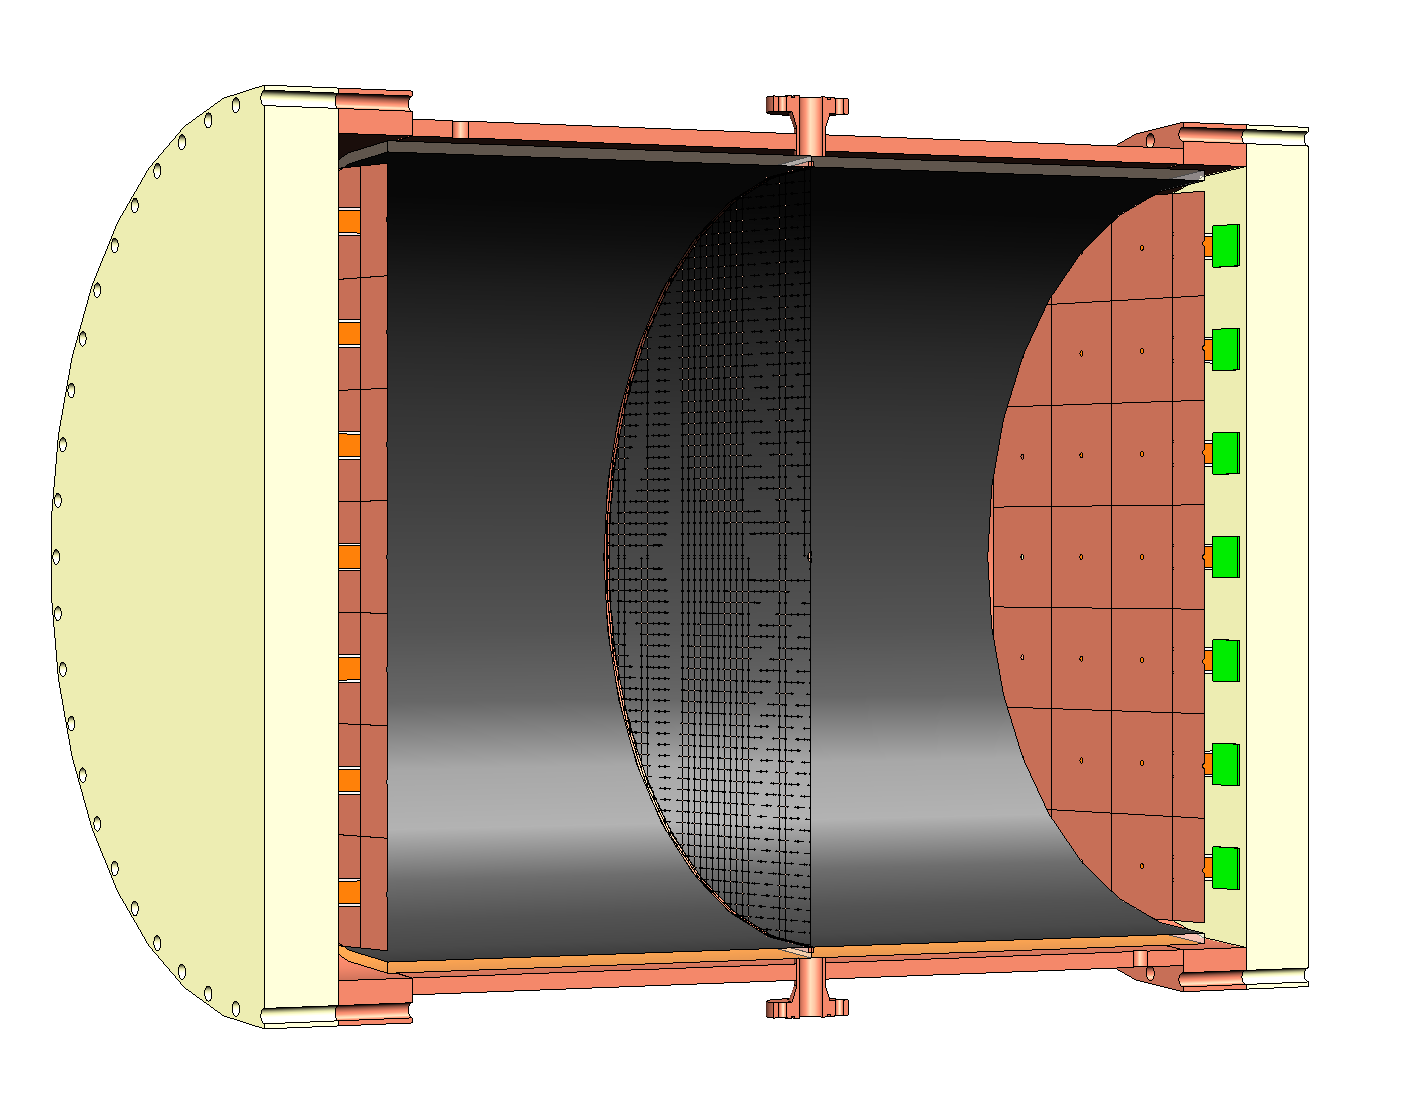
\includegraphics[width=0.4\columnwidth]{pic/fig1.png}
    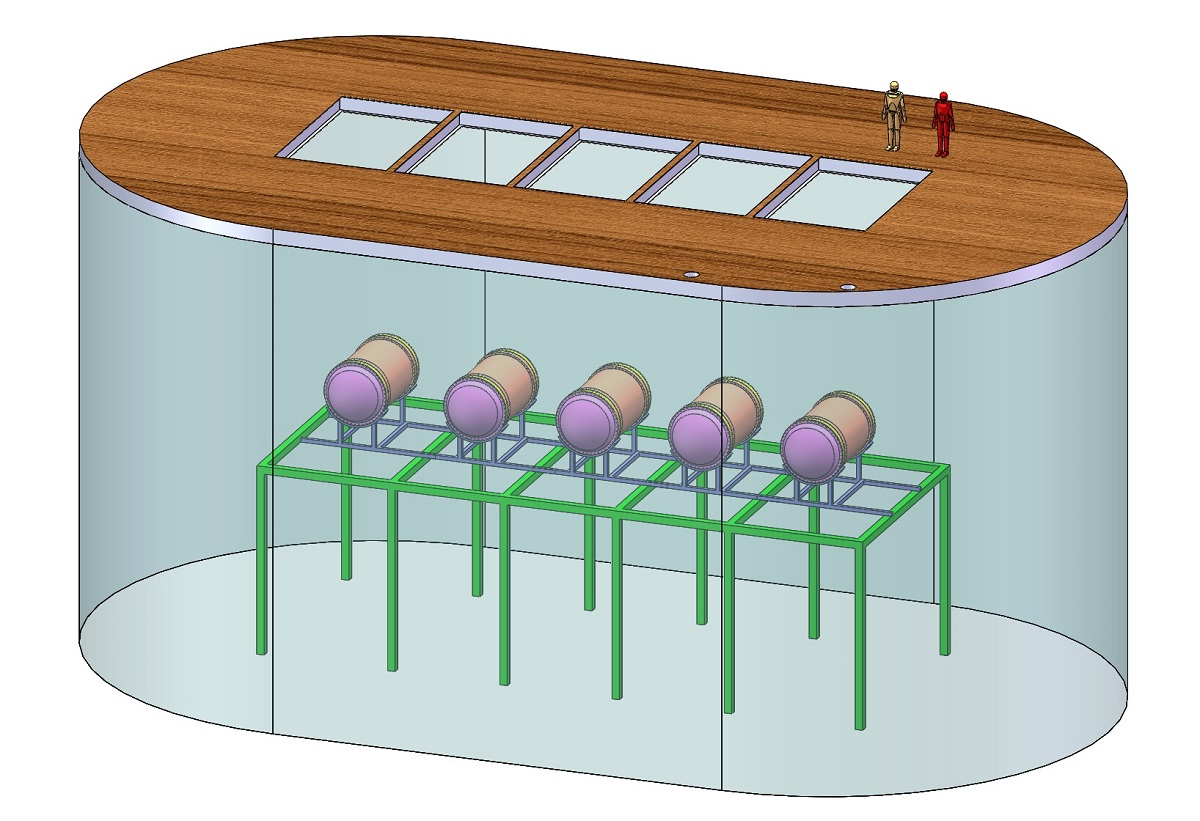
\includegraphics[width=0.4\columnwidth]{pic/fig2.jpg}
    \caption{左图:PandaX-III时间漂移室结构示意图。右图:5个TPC被放置在屏蔽水池示意图。}
    \label{fig:detector}
\end{figure}
    
探测器主体是一个内高2米,内径1.5米的柱形压力铜罐,使用了高纯度无氧铜制作,总容积约3.5m$^3$。在铜罐中心部分有圆形网状极板,在铜罐内壁有99个圆形铜环,铜环之间以及铜环与内壁之间使用聚四氟乙烯(PTFE)做隔离和支撑,铜环,极板之间形成场笼,提供延罐体轴心方向,强度为1kV/cm的漂移电场。铜罐壁自身厚度约30mm,两端厚度约150mm,整体放置于在如图\ref{fig:detector}右侧的水池中,利用超纯水来屏蔽来自周围环境的本底射线。同时整体实验位于中国锦屏地下实验室中,利用隧道上方2500米厚的山岩屏蔽宇宙射线。对于探测器自身材料产生的本底射线,PandaX-III实验通过适当的材料选择和探测器构造来降低这部分背景干扰。本文第\ref{chapter:section:background}章主要介绍了使用Geant4模拟并分析探测器材料所带来的具体影响。

\section{电子学读出}


% vim:ts=4:sw=4
